\documentclass{article} % For LaTeX2e
\usepackage{nips15submit_e,times}
\usepackage{hyperref}
\usepackage{url}
\usepackage{graphicx}
\usepackage{mathtools}
\usepackage{float}
\usepackage[inline]{enumitem}
\usepackage{multirow}
\usepackage[toc,page]{appendix}
\usepackage{caption} 
\captionsetup[table]{skip=10pt}
\usepackage{cite}
\usepackage{csquotes}
\usepackage{amsmath}
\DeclareMathOperator*{\argmax}{arg\,max}


%\documentstyle[nips14submit_09,times,art10]{article} % For LaTeX 2.09


\title{COMPGI19 Assignment 3 Report}

\author{
Reece Doyle
\And
Navid Hallajian \\
\And
Kapileshwar Syamasundar \\
\And
Oliver Tun \\
}

\newcommand{\fix}{\marginpar{FIX}}
\newcommand{\new}{\marginpar{NEW}}

\nipsfinalcopy % Uncomment for camera-ready version

\begin{document}

\maketitle

\section{Gradient Checking}
By using backpropagation, we are calculating gradients for blocks and then reusing them as intermediate results in the gradient calculations for other blocks; this saves on a substantial amount of computation time. If we were to use the gradient approximation for each block with respect to the loss function, we would not be making this computational saving.

Suppose we combine these two approaches and use the gradient approximation formula for calculating the gradient of each block with respect to the upstream block, and then use backpropagation to calculate the derivation of each block with respect to the loss function. Calculating the gradient for a model would involve multiplying many of these estimated gradients together, each of which has a slight error, potentially resulting in the introduction of errors significant enough to change the classification.

One such deviation of the approximated gradient from that calculated through backpropagation is $1.2714735930785537 \times 10^{-8}$ for the Dot block.

\section{Sum-of-Word-Vectors Model}

\subsection{Blocks}

\begin{enumerate}

\item Dot product

\[ z \frac{\partial {\mathbf{x} \cdot \mathbf{y}}}{\partial{\mathbf{x}}} = z \mathbf{y}  \]

\[ z \frac{\partial {\mathbf{x} \cdot \mathbf{y}}}{\partial{\mathbf{y}}} = z \mathbf{x} \]

\item Sigmoid

\[z \frac{\partial \text{sigmoid} (x)}{\partial{x}} =  \text{sigmoid}(x) (1 - \text{sigmoid}(x)) z\]

\item Negative log-likelihood

\[ \frac{\partial \mathcal{L}(f_{\theta}(x), y)}{\partial{f_{\theta}(x)}} = \frac{-y}{f_{\theta}(x)} + \frac{1 - y}{1 - f_{\theta}(x)} \]

\item Regularisation

\[ \frac{\partial \lambda * \frac{1}{2} {|| \theta ||}^2_2}{\partial \theta} = \theta \]

\end{enumerate}

\subsection{Model}

We get an error of $7.042 \times 10^{-11}$ for the sum of words vector model.

\subsection{Grid Search and Evaluation}

To determine the best choice of parameters for the sum of words model, we first performed  coarse grid searches over a large range of possible values for the word vector dimension, vector regularisation strength and learning rate. We found that the best results occurred when the parameters were bound between the following ranges:

\begin{itemize}

\item Word vector dimensions: $[7, 11]$
\item Vector regularisation strength: $(0, 1]$
\item Learning rate: $(0, 1)$

\end{itemize}

Having established this, we were then able to perform a more refined grid search. Due to computational limitations (and in the interest of keeping experiments fair), training was limited to 50 epochs per set of parameters. Our results are summarised in table 1:

\begin{table}[htb]
\centering
\resizebox{\textwidth}{!}{
%\begin{tabular}{|l|l|l|l|}
\begin{tabular}{|c|c|c|c|}
\hline
Word vector dimension & Vector regularisation strength & Learning rate & Error on development set \\ \hline
10 & 0.05 & 0.05 & 40.279627163781626 \\ \hline
10 & 0.01 & 0.01 & 40.279627163781626 \\  \hline
8 & 0.005 & 0.05 & 40.3462050599201 \\  \hline
7 & 0.05 & 0.005 & 76.49800266311586 \\  \hline
8 & 0.05 & 0.05 & 40.3462050599201 \\  \hline
7 & 0.005 & 0.01 & 74.56724367509987 \\  \hline
8 & 0.01 & 0.05 & 40.279627163781626 \\  \hline
10 & 0.05 & 0.005 & 76.43142476697736 \\  \hline
8 & 0.05 & 0.005 & 76.83089214380826 \\ \hline
10 & 0.005 & 0.01 & 40.279627163781626 \\  \hline
7 & 0.01 & 0.05 & 40.3462050599201 \\ 	 \hline
10 & 0.05 & 0.01 & 75.89880159786951 \\  \hline
10 & 0.01 & 0.05 & 40.279627163781626 \\ \hline
7 & 0.01 & 0.01 & 75.69906790945407 \\ \hline
9 & 0.01 & 0.01 & 75.43275632490013 \\ \hline
9 & 0.05 & 0.01 & 76.03195739014647 \\ \hline
7 & 0.05 & 0.05 & 40.21304926764314 \\ \hline
9 & 0.01 & 0.005 & 75.23302263648469 \\ \hline
10 & 0.01 & 0.005 & 75.09986684420772 \\ \hline
9 & 0.05 & 0.05 & 40.279627163781626 \\ \hline
9 & 0.05 & 0.005 & 76.89747003994674 \\ \hline
7 & 0.05 & 0.01 & 75.96537949400799 \\ \hline
9 & 0.01 & 0.05 & 40.279627163781626 \\ \hline
7 & 0.01 & 0.005 & 76.09853528628496 \\ \hline
7 & 0.005 & 0.005 & 40.21304926764314 \\ \hline
9 & 0.005 & 0.005 & 74.23435419440746 \\ \hline
10 & 0.005 & 0.05 & 40.279627163781626 \\ \hline
8 & 0.01 & 0.005 & 75.76564580559254 \\ \hline
8 & 0.005 & 0.01 & 74.63382157123834 \\ \hline
8 & 0.05 & 0.01 & 75.69906790945407 \\ \hline
7 & 0.005 & 0.05 & 40.279627163781626 \\ \hline
8 & 0.005 & 0.005 & 74.43408788282291 \\ \hline
10 & 0.005 & 0.005 & 75.03328894806924 \\ \hline
9 & 0.005 & 0.01 & 74.83355525965379 \\ \hline
9 & 0.005 & 0.05 & 40.3462050599201 \\ \hline
8 & 0.01 & 0.01 & 74.43408788282291 \\	 \hline
\label{mainresults}
\end{tabular}
}
\caption{Grid search on Sum of Words model}
\end{table}

Our best parameters for the sum of word vectors model were:

\begin{itemize}

\item Word vector dimension: $9$
\item Vector regularisation strength: $0.05$
\item Learning rate: $0.005$

\end{itemize}

These parameters gave a development set accuracy of $76.89\%$.

From the results we observed that the model was very sensitive to the learning rate used during training. Keeping all other parameters unchanged, at a learning rate of 0.05 the development accuracy dropped to $40.28\%$. We also observed that the value of the regularisation strength did not have a large effect on the development set accuracy; changing it to one order of magnitude lower (0.005) only decreased the accuracy by $2\%$.

\subsection{Loss Analysis}

To help analyse the performance of the model on a per epoch basis, the figure below shows the training loss over epochs. As expected, the training loss decreased between epochs but this rate of change was not linear and appears to plateau during the higher epochs. 
After 300 epochs, the training loss was $25600$.

\begin{figure}[H]
\centering
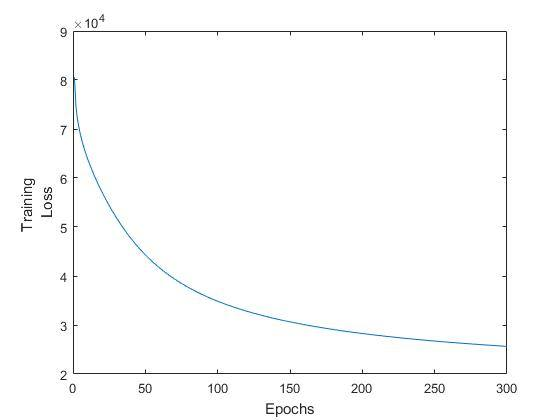
\includegraphics[width=0.75\textwidth]{graphics/tloss.jpg}
\caption{Training loss over epochs.}
\end{figure}

\begin{figure}[H]
\centering
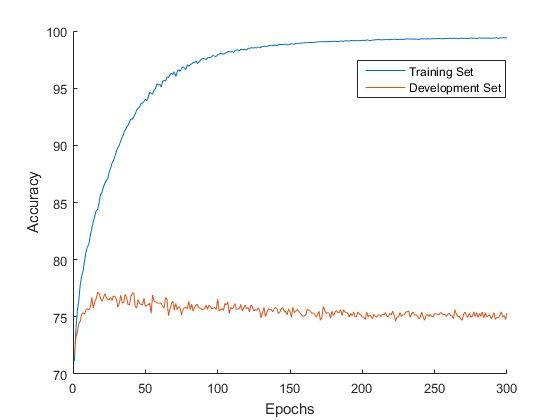
\includegraphics[width=0.75\textwidth]{graphics/tdloss.jpg}
\caption{Training and development accuracy over epochs.}
\end{figure}

Having observed the change in training loss, it is no surprise that the training set accuracy continuously increases over epochs until the plateau close to $100\%$ (see Figure 1). The accuracy on both sets is shown in Figure 2, the change of the development set accuracy is not immediately obvious due to the fluctuations. It can be seen that after the initial increase in development accuracy, it quickly plateaus and then gradually decreases. The figure below demonstrates this. From this decrease in development accuracy and the large variance between the training and development accuracies, we can conclude that the model suffers from overfitting.

\begin{figure}[H]
\centering
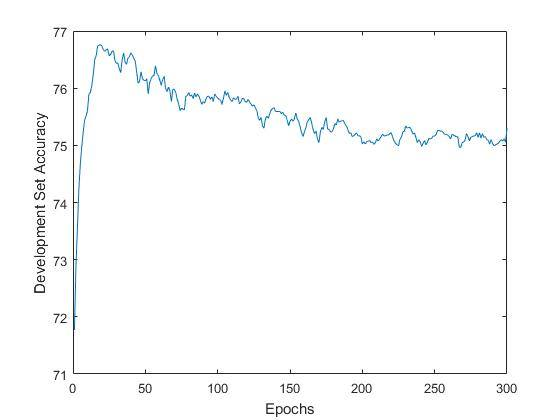
\includegraphics[width=0.75\textwidth]{graphics/devaccuracy.jpg}
\caption{Training and development accuracy over epochs.}
\end{figure}

\subsection{t-SNE Visualisation}

We round the values of the predictions to get a binary classification. Blue data points represent a positive classification and orange is negative. Due to the run time of the t-SNE program, we sample 10000 data points.

\begin{figure}[H]
\centering
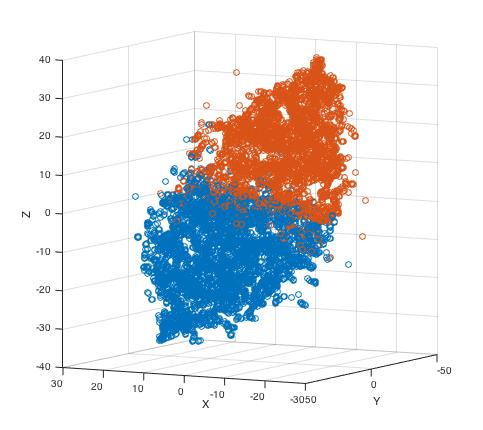
\includegraphics[width=0.75\textwidth]{graphics/tsneplot.jpg}
\caption{t-SNE visualisation.}
\end{figure}

\section{Recurrent Neural Networks}

\subsection{Blocks}

\begin{enumerate}

\item Matrix-vector multiplication

\[\mathbf{z} \frac{\partial \mathbf{W} \mathbf{x}}{\partial \mathbf{x}}  = \mathbf{W}^{\text{T}} \mathbf{z}\]

\[\mathbf{z} \frac{\partial \mathbf{W} \mathbf{x}}{\partial \mathbf{W}}  = \mathbf{z} \otimes \mathbf{x}\]

\item tanh

Note that $x$ refers to a single element in the vector $\mathbf{x}$. The element wise application of $\text{tanh}$ would apply this function to each element of $\mathbf{x}$.

\[ \frac{\partial \text{tanh}(x)}{\partial x} = 1 - \text{tanh}^2(x) \]

\end{enumerate}

\subsection{Model}

We get an error of $6.301 \times 10^{-11}$ for the RNN model.

\subsection{Grid Search, Initialisation, Evaluation and Comparison}

Due to the computational complexity of the RNN model, running extensive grid searches for tuning the hyper parameters was not as practical when compared to the sum of words model. We explored 2 variants of early stopping when training but eventually chose to stick with running each selection of hyperparameters for 50 epochs, in order to compare performance against the sum of words model. The first variant we experimented with was where training would stop when the development accuracy decreased between epochs while the second variant only checked for this condition every 5 epochs. Due to the fluctuations in development accuracy, it was determined that this would perhaps not have been the most optimal way to tune the parameters and that a static number of epochs was more indicative. Given the time constraints, we implemented a random search instead. Our best parameters for the RNN model were:

\begin{itemize}

\item Word vector dimension: $8$
\item Hidden dimension: $7$
\item Vector regularisation strength: $7.786 \times 10^-5$
\item Matrix regularisation strength: $9.741 \times 10^-5$
\item Learning rate: $0.001$

\end{itemize}

These choices of parameters for this model gave a development set accuracy of $76.76\%$.

\section{Sky's the Limit}

\subsection{Dropout regularisation}

Dropout regularisation works by dropping connections between nodes of the neural network during training time, changing the topology of the neural network between each epoch. After training is completed, the neural network reconnects all of the nodes as normal.

Dropout regularisation reduces the amount of overtraining experienced by the neural network and prevents co-adaptation  from occurring. It does this by having the approximate effect of training an exponentially large amount of smaller and more focused neural nets, combining them into a larger neural net during test time.

The implementation involved adding to the Blocks class by implementing dropout blocks. Each dropout block is given a probability and randomly generates a double between 0 and 1 on each update function. If the randomly generated value is greater than the probability value given, the dropout block will return a zero vector when the forward function is called and perform no actions when the backward function is called. Otherwise, the dropout block will act transparently and pass values between nodes as if it did not exist.

During testing time, the weights from the dropout model are copied into a normal SumOfVectors model (no dropout blocks) which is used for evaluation. Using the optimal parameters that we obtained for the original SumOfVectors model, we achieve an accuracy of $77.1\%$ on the development set.

\subsection{Multiplication-of-Word-Vectors Model}

This model was implemented by judging the score of a sentence by taking the element-wise product of the outputs produced by the nodes as opposed to summing them as performed by the sum-of-word-vectors model. 

Upon comparison of the two models, it appeared that the sum model performed more effectively than the multiplicative model over a period of 10 epochs and 100 epochs. The accuracy on the development set provided by the multiplication model was $59.25\%$, lower than what we achieved for sum-of-word-vectors.

\subsection{Long Short-Term Memory RNN (LSTM)}

\subsubsection{Blocks}

\begin{enumerate}

\item Concat

This block represents the vertical concatenation of two vectors to one vector. The backwards gradient is calculated by splitting the upstream gradient into two vectors that are the same length as the two arguments.

\item

Per-element sigmoid

This block applies the sigmoid function to each element of a vector to produce a new vector. The derivative for each element is equivalent to the derivative given for sigmoid in 2.1.2.

\item

Element-wise vector multiplication

This block takes two vector blocks as arguments and applies element-wise multiplication, similar to the Hadamard product of matrices. Note that in the derivative given below, $\odot$ is the element-wise multiplication operator.

\[
\mathbf{z} \frac{\partial \mathbf{x} \odot \mathbf{y}}{\partial \mathbf{x}} = \mathbf{z} \odot \mathbf{y}
\]

\end{enumerate}

\subsubsection{Model}

LSTMs are capable of learning long-term dependencies. One problem with standard RNNs is that with each new word, the impact of a prior word on the current hidden state becomes increasingly diluted, meaning it can be hard to learn dependencies between distant words in a tweet. One example in which it is useful to learn such a dependency is the tweet

\begin{displayquote}
I really don't, and I'm not just saying this because it's a great example and I couldn't think of anything else, like Scala.
\end{displayquote}

In this example, it is useful to remember that \emph{don't} occurred before \emph{like} when conducting sentiment analysis. The LSTM uses an additional cell state to which it can write information about the word vectors and hidden weights to help form these dependencies.

Unfortunately, we found that the computational cost of running the LSTM model too high to complete training. However, we expect it to perform better.

\subsection{Loading pre-trained word2vec vectors}

When we encounter a word for the first time, we generate its vector representation as a set of random values. wor2vec is a tool that is able to create representative word embeddings given a corpus. We approached two different methods of using these embeddings. In both approaches our intuition is that representative embeddings will cause our model to converge to the optimum development accuracy faster since it would not need as many epochs to learn word embeddings as compared to a random embedding (due to starting off in a better position on the error surface).

To use word2vec, we used a Python interface over the original C library to pass in our training data and generate a CSV file with words and their vector representations. We read this file into our model's lookup table.

In the first approach we treated the embeddings as constant by storing them in the fixed hash map and changing the \texttt{wordToVector} function to first see if it has a representation in the fixed hash map before adding a new trainable vector to the trainable hash map. This is based on the assumption that close vectors as defined by word2vec would share similar sentiment.

In the second approach, the embeddings were trainable. Here we thought that although similar words may have similar sentiment, they only serve as a good initial guess since word2vec cares about similarity in meaning primarily (by looking at the context in which words are used) and not sentiment. This performed better than the first approach, achieving $75.77\%$ accuracy on the development set over 100 epochs.

Further work could be done with this approach by using a larger corpus to train word2vec to help minimise the issue of unseen words. 

\bibliography{references}{}
\bibliographystyle{plain}

\end{document}